\documentclass{standalone}

\usepackage{pgfplots,tikz,amsmath}
\begin{document}
    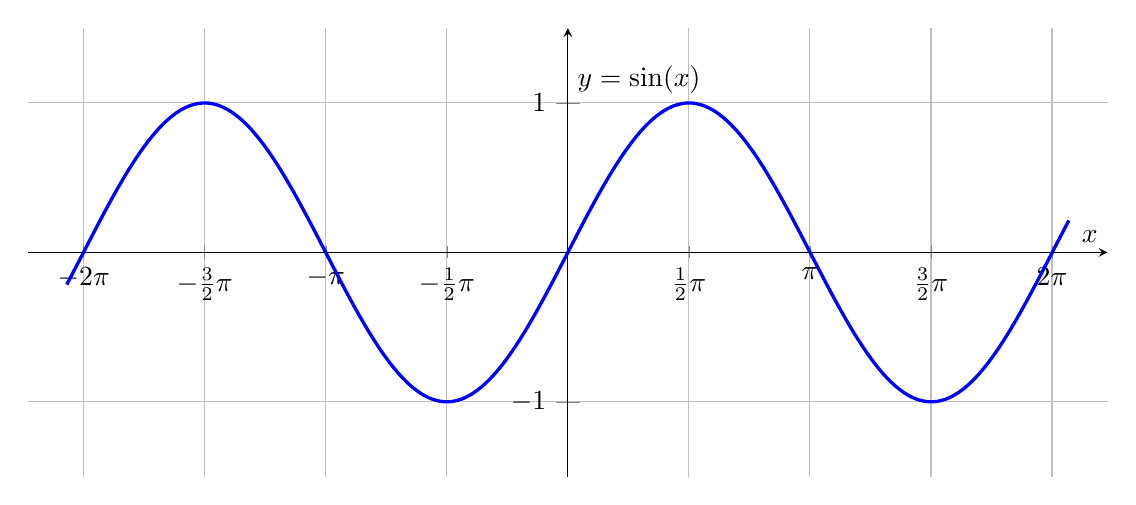
\begin{tikzpicture}
        \begin{axis}[axis lines=center, xlabel={$x$}, xmin=-7, xmax=7,
                ymin=-1.5, ymax=1.5, ytick={-1,1}, xtick={-6.28, -4.71, -3.14, -1.57,
                1.57, 3.14, 4.71, 6.28},
            xticklabels={$-2\pi$,$-\frac{3}{2}\pi$,$-\pi$,$-\frac{1}{2}\pi$,$\frac{1}{2}\pi$,$\pi$,$\frac{3}{2}\pi$,$2\pi$},
        grid, xscale=2]
            \addplot[smooth, very thick, color=blue, domain=-6.5:6.5, samples=100] {sin(deg(x))};
            \draw (axis cs:0,1) node[anchor=south west]{$y = \sin(x)$};
        \end{axis}
    \end{tikzpicture}
\end{document}
